
\documentclass[12pt, a4paper]{article}

\usepackage{pdflscape} % pdflscape
\usepackage{graphicx}
\graphicspath{ {./images/} }
%Tarih Ekleme
\usepackage[ddmmyyyy]{datetime}
\renewcommand{\dateseparator}{.}
\renewcommand{\figurename}{Şekil}
\renewcommand{\refname}{Kaynakça}
\usepackage{hyperref}
\usepackage{natbib}

\title{\bf\fontsize{12pt}{14pt}\selectfont KÜTAHYA SAĞLIK BİLİMLERİ ÜNİVERSİTESİ \\ MÜHENDİSLİK VE DOĞA BİLİMLERİ FAKÜLTESİ}
\date{}


\begin{document}
	\maketitle
	
	\begin{center}
		
\includegraphics[width=0.25\linewidth]{ksbu.jpg}
	\end{center}	
	\begin{center}
		\vspace{1cm} 
	\end{center}
	\begin{center}
		\title{\bf\fontsize{12pt}{14pt}\selectfont Final Raporu}
	\end{center}
	\begin{center}
		\vspace{1cm} % Vertical space of 1cm
	\end{center}
	\begin{center}
		
		\author{\bf\fontsize{12pt}{14pt}Halil Şimşek \hspace{1,5cm}2218111004}
		
		\begin{center}
			\vspace{1cm} 
		\end{center}
		\date{\textbf{\today}}
	\end{center}
	\newpage
	
\section{PostgreSQL Fonksiyonları ve Veri Girişi}

Proje süreci kapsamında bu hafta, PostgreSQL'de fonksiyonların öğrenilmesi ve uygulanması üzerine çalışmalar gerçekleştirilmiştir. Veritabanı katmanında, kitap ekleme ve listeleme işlemleri başarılı bir şekilde tamamlanmıştır. Fonksiyonların öğrenilmesi aşamasında, Murat Yücedağ'ın YouTube kanalından faydalanılmıştır. \cite{kanal:isim} \newline

	 \begin{figure}[htbp]
	\centering
	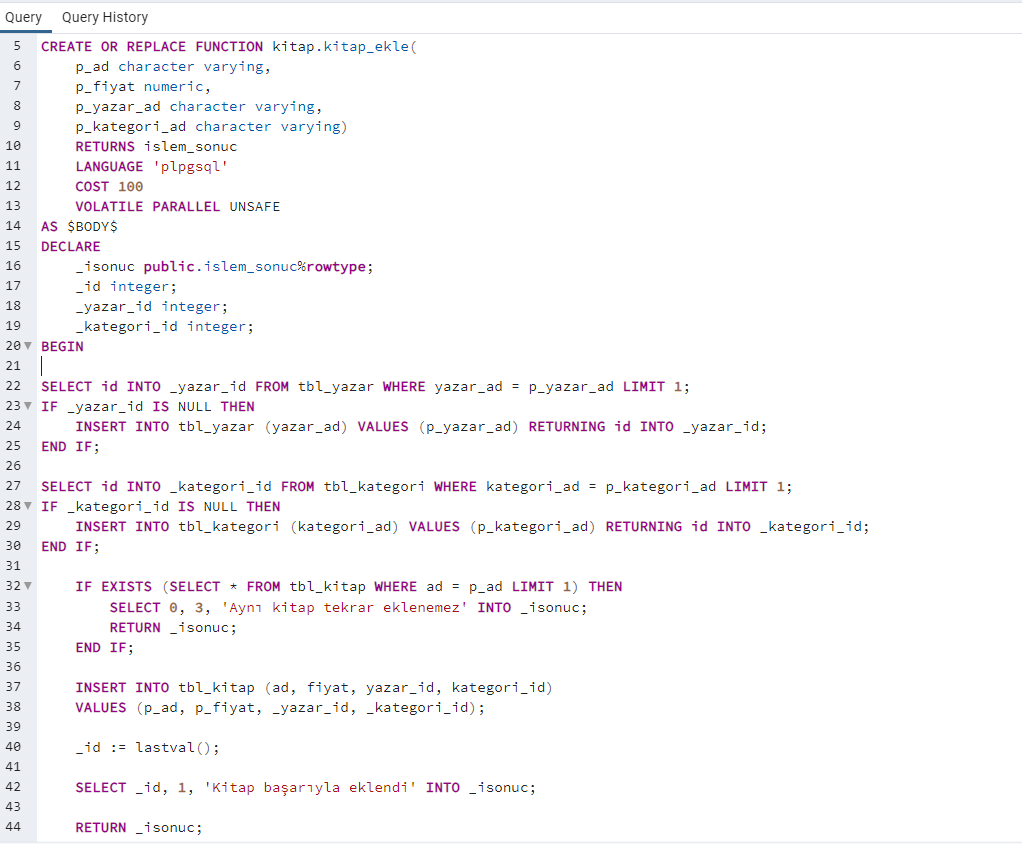
\includegraphics[width=15cm, height=15cm]{ekleFonksiyon.png}
	\caption{PostgreSql'de Fonksiyon Kullanımı}
	\label{fig:fonksiyon}
\end{figure}

\subsection{Type Kullanımının Avantajları}

\begin{figure}[htbp]
	\centering
	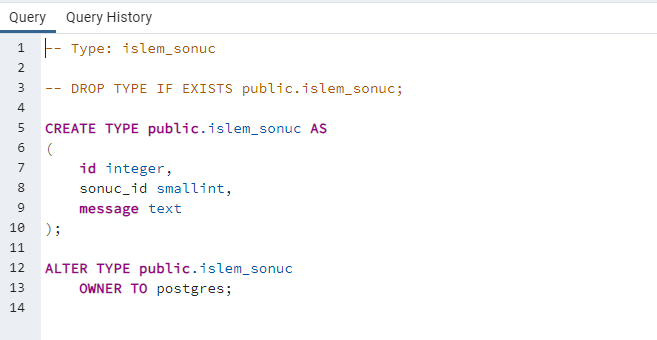
\includegraphics[width=\textwidth, height=8cm]{type.png}
	\caption{Type Kullanımının Gösterimi}
	\label{fig:type}
\end{figure}

\begin{itemize}
	\item Daha İyi Tip Güvenliği: Geri dönüş değeri olarak tip kullanmak, belirli bir türün dönmesini beklediğinizde daha sağlam bir tip güvenliği sağlar. Tip belirtmek, beklenmeyen veri türü dönüşlerine karşı kodunuzu korur ve hataları önler.
	\item Kod Okunabilirliği ve Anlaşılabilirlik: Fonksiyonun geri dönüş değerini belirtmek, kodun daha okunabilir ve anlaşılabilir olmasını sağlar. Fonksiyonun ne tür bir değer döndüreceği hakkında açık bir bilgi verir, bu da kodu anlamayı ve bakımını daha kolay hale getirir.
	\item Dökümantasyon ve API Uyumluluğu: Geri dönüş değerini belirtmek, fonksiyonun dış dünyayla etkileşimini açıklığa kavuşturur. API'ler arasında tutarlılık sağlar ve dış kullanıcılar veya diğer geliştiriciler için fonksiyonun nasıl kullanılacağı hakkında açık bir belge sağlar.
	\item Veri Doğrulama ve Kısıtlamalar: PostgreSQL'de tip kullanarak, geri dönüş değeri üzerinde veri doğrulama ve kısıtlamalar uygulanabilir. Bu, istenmeyen değerlerin dönmesini önler ve veri bütünlüğünü korur.
\end{itemize}

\newpage
Aynı zamanda ekleme,silme,güncelleme gibi ortak işler için bir type oluşturuldu. Bu type sayesinde yapılan işlemlere göre kullanıcıya bir mesaj verilebilecek.
Ekleme fonksiyonunu kullanarak veri tabanındaki kitap sayısı da arttrırılmıştır. 
Type Araştırmasında Chatgpt'den yararlanılmıştır. \cite{chatgpt}

	\section{ASP.NET MVC Model Katmanı}

\begin{figure}[htbp]
	\centering
	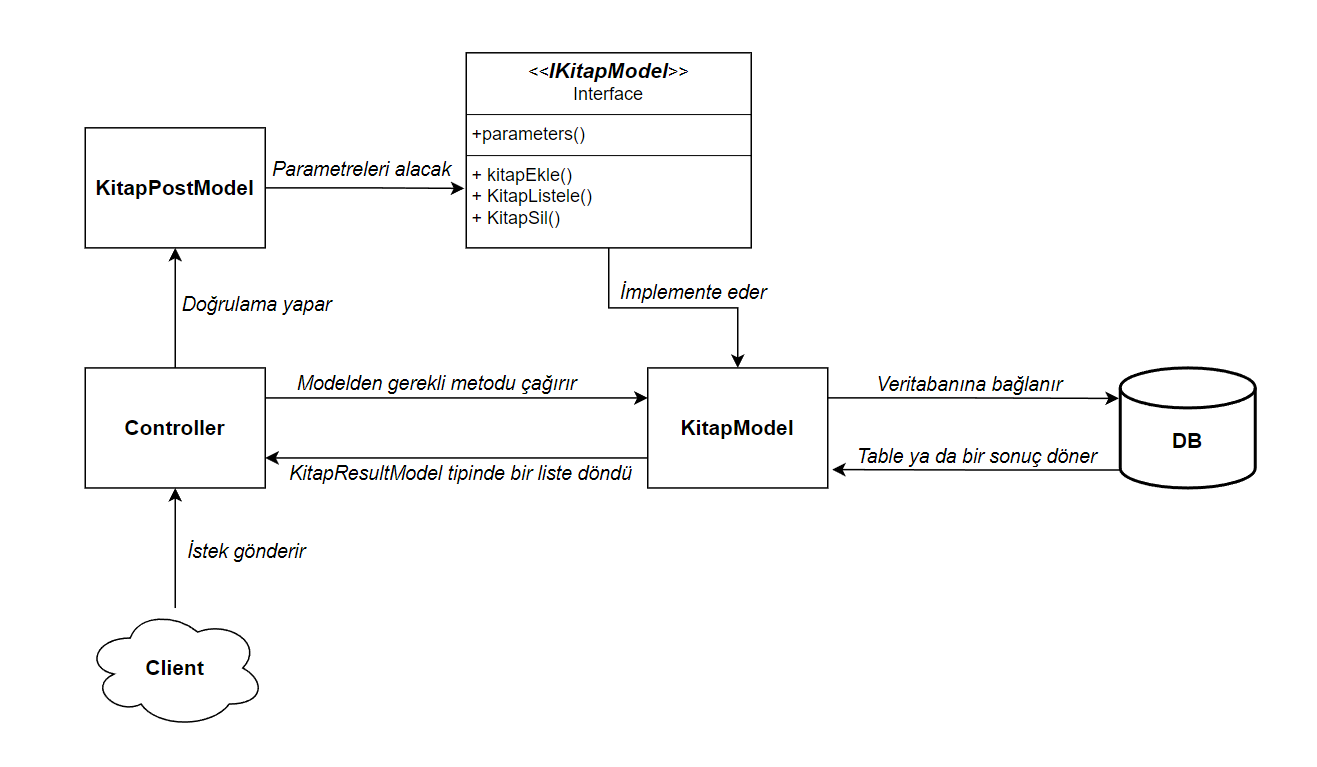
\includegraphics[ width=\textwidth, height=10cm]{mvcSistem.png} 
	\caption{Model Katmanının İşleyişi}
	\label{fig:type}
\end{figure}

\newpage
\subsection{IKitapModel Arayüzü}
Bu arayüz, kitaplarla ilgili işlemlerin sözleşmesini tanımlar. Yani, kitap listeleme ve kitap ekleme gibi işlevlerin prototiplerini içerir.
KitapListe metodu, kitap listeleme işlemi için gerekli parametreleri (KitapPostModel) alır ve sonuç olarak bir KitapResultModel listesi döndürür. Bu metod, veritabanından kitap listesini almak için kullanılır.
\newline
\vspace{8mm}

\begin{figure}[htbp]
	\centering
	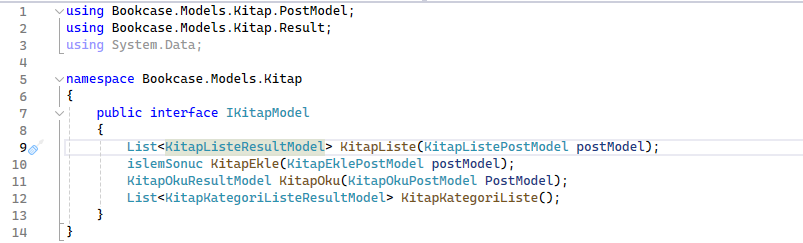
\includegraphics[ width=\textwidth, height=6cm]{IKitapModel.png} 
	\caption{IKitapModel İnterface}
	\label{fig:type}
\end{figure}

\subsection{KitapModel Sınıfı}
IKitapModel arayüzünü uygular (implement eder) ve bu arayüzde tanımlanan metodların somut davranışlarını içerir.
KitapListe metodunun somut uygulaması, PostgreSQL veritabanına bağlanır, bir SQL sorgusu çalıştırır ve sonuçları bir KitapResultModel listesine dönüştürür.Veritabanı bağlantısı ve sorgu işlemleri için NpgsqlConnection ve NpgsqlCommand nesnelerini kullanır.
\newline

\begin{figure}[htbp]
	\centering
	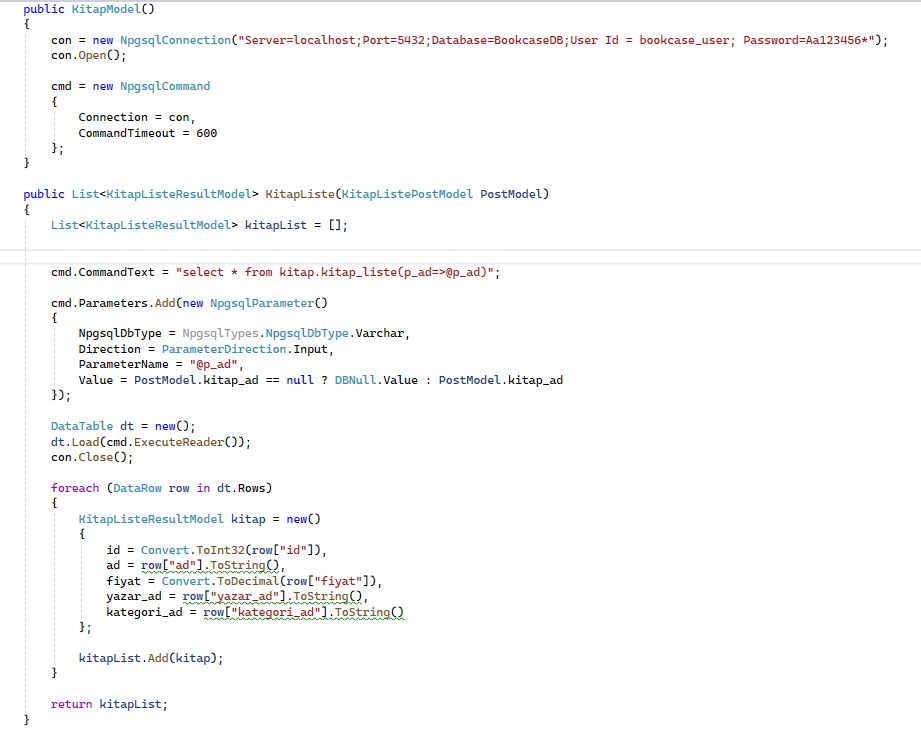
\includegraphics[ width=\textwidth, height=17cm]{KitapModel.png} 
	\caption{KitapModel Sınıfının Kodları}
	\label{fig:type}
\end{figure}
\newpage

\subsection{KitapPostModel Sınıfı}	
Kullanıcıdan alınan verileri taşımak için kullanılır. Bu model, kitap listeleme işlemi sırasında kullanıcı tarafından sağlanan verileri (örneğin, bir kitap adı) içerir.IValidatableObject arayüzünü uygular ve Validate metodu ile modelin kendini doğrulamasını sağlar.Bu arabirim, bir sınıfın Validate metodunu uygulamasını gerektirir.\newline Bu metod, sınıfın kendi doğrulama mantığını içerir ve sınıfın durumunu değerlendirir. Validate metodu, geçerli bir nesne durumunu döndürdüğünde, sınıfın geçerli olduğu anlamına gelir. Geçerli bir nesne durumu döndürülmediğinde ise, sınıfın geçerliliği başarısız olur ve bu durumda hata mesajları veya hata listeleri ile birlikte geçerli olmayan nesne durumu döndürülebilir.

ASP.NET MVC veya ASP.NET Core MVC projelerinde, özellikle model doğrulaması yapmak için sıklıkla IValidatableObject arabirimi kullanılır. Bir modelin belirli doğrulama kurallarını uygulamak ve bu kurallara uygunluğunu kontrol etmek için IValidatableObject arabirimi uygulanabilir. Bu, gelen verilerin doğruluğunu sağlamak için önemli bir mekanizmadır ve hatalı girişlerin önlenmesine yardımcı olur.
\newline
\newline

\begin{figure}[htbp]
	\centering
	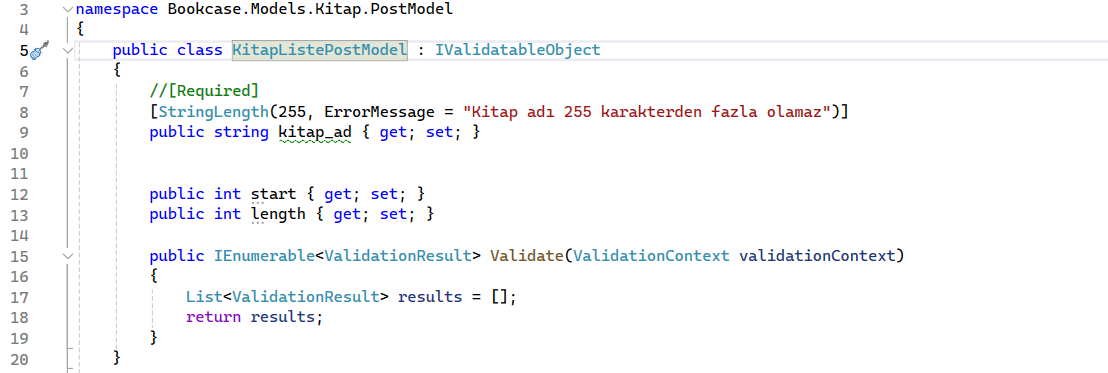
\includegraphics[ width=\textwidth, height=6cm]{KitapPostModel.png} 
	\caption{KitapPostModel Sınıfının Kodları}
	\label{fig:type}
\end{figure}

\newpage	

\subsection{KitapResultModel Sınıfı}	
Veritabanından dönen sonuçları temsil eder. Her bir KitapResultModel nesnesi, bir kitap kaydının id, ad, fiyat, yazarAd, kategoriAd gibi özelliklerini içerir.
\newline \newline

\begin{figure}[htbp]
	\centering
	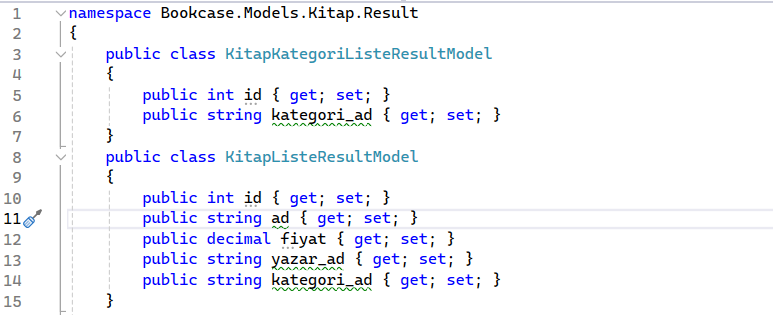
\includegraphics[ width=\textwidth, height=6cm]{KitapResultModel.png} 
	\caption{KitapResultModel Sınıfının Kodları}
	\label{fig:type}
\end{figure}



\subsection{Controller}	
MVC'nin Controller bileşenidir ve kullanıcı isteklerini yönetir.
Index metodu, uygulamanın ana sayfasını döndürür ve genellikle kullanıcıya HTML içeriği sunar.
kitapListe metodu, bir HTTP POST isteği ile çağrıldığında, KitapListePostModel tipindeki veriyi alır, modelin geçerliliğini kontrol eder ve KitapModel üzerinden kitap listesini çeker. Daha sonra bu listeyi JSON formatında istemciye (web tarayıcısına) geri döndürür.
\newpage
\begin{figure}[htbp]
	\centering
	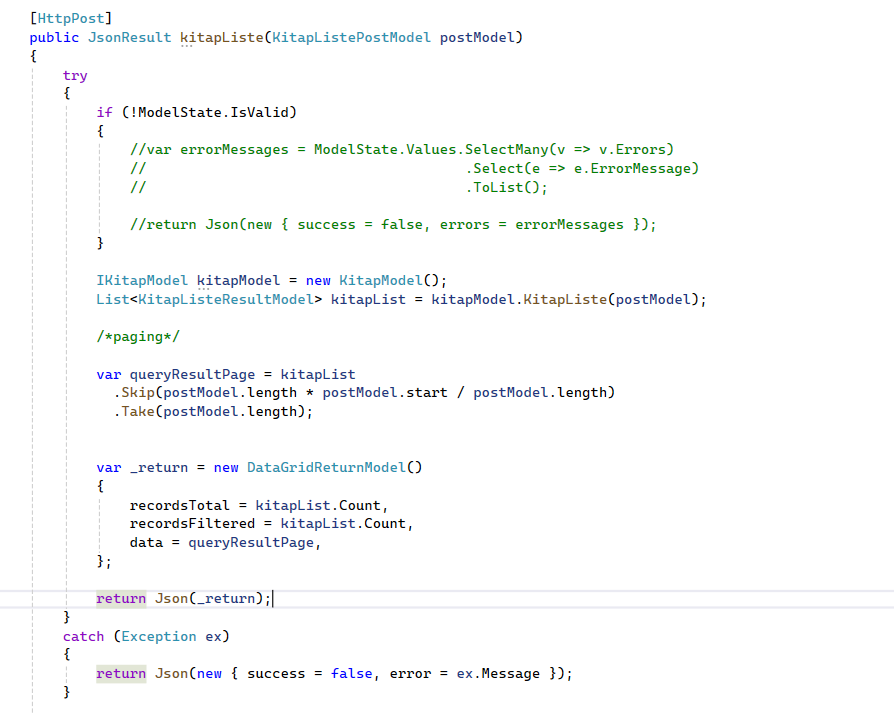
\includegraphics[ width=\textwidth, height=15cm]{Controller.png} 
	\caption{Controller Sınıfının Kodları}
	\label{fig:type}
\end{figure}
\newpage

\section{Listeleme İşleminin Gerçekleştirilmesi}

Listeleme işlemi yapılırken hazır grid kullanılmıştır. Grid bu websiteden alınmıştır \cite{datatables}. 
 Bootstrap kütüphanesinden yararlanılmıştır. Bootstrap hakkındaki araştırmalar ve öğrenimlerde \cite{bootstrap} sitesinden yararlanılmıştır. Listelenen gridin son hali şekil:9 da bulunmaktadır.


\begin{figure}[htbp]
	\centering
	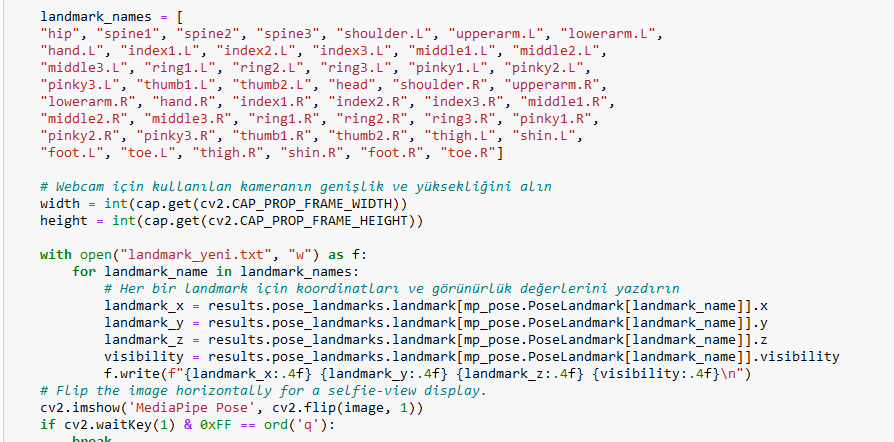
\includegraphics[ width=\textwidth, height=11cm]{liste.png} 
	\caption{Listelenen Veriler}
	\label{fig:type}
\end{figure}

\newpage
\section{Detay Butonunun Eklenmesi}

Gerçekleştirilen listeleme işlemi sonrasında bir detay butonu eklendi. Bu detay butonunun amacı aslında bu yapılan listemedeki sütun sayılarından cok daha fazlasına sahip tablolarda ana ekranda gösterilemeyen bilgileri detay ekranında göstererek düzen sağlamayı hedefler \cite{jivochat2024}. 
\newline

\begin{figure}[htbp]
	\centering
	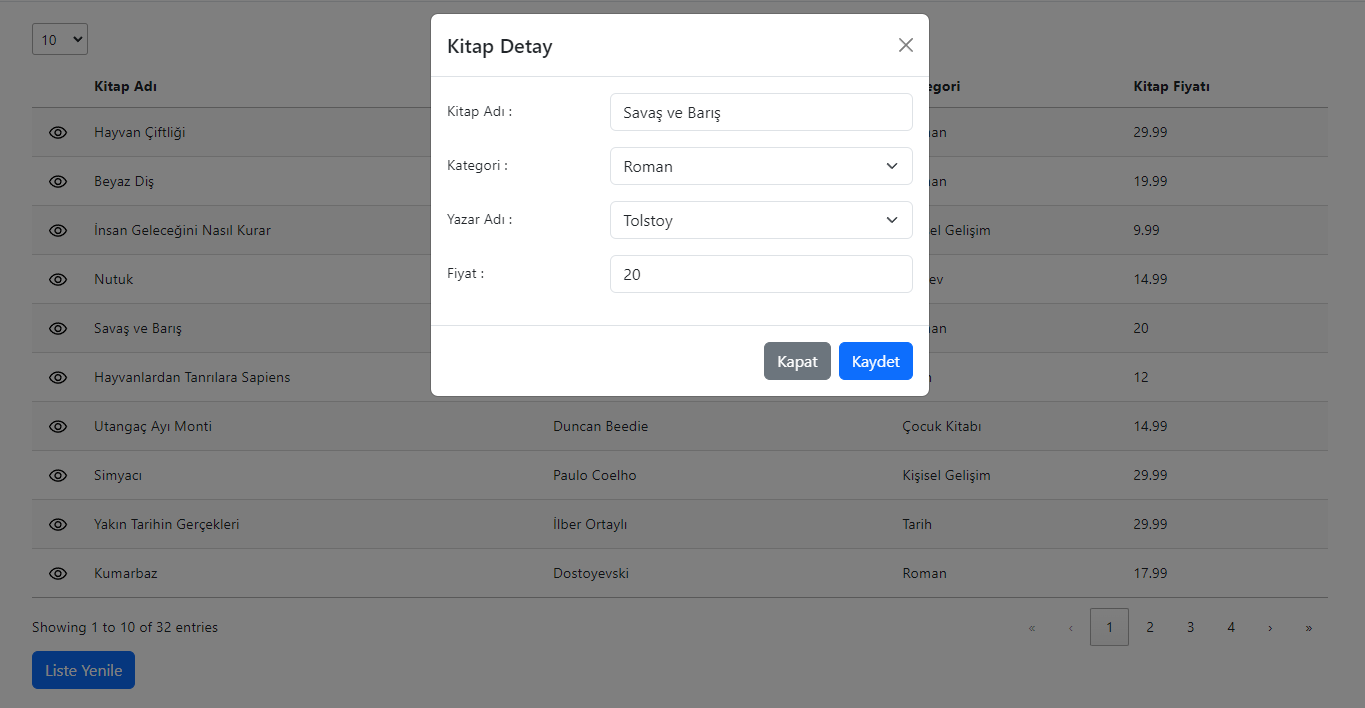
\includegraphics[ width=\textwidth, height=9cm]{detay.png} 
	\caption{Detay Popup}
	\label{fig:type}
\end{figure}

Bu Bootstrap modal örneği, kullanıcıların bir detayı incelemek veya düzenlemek için bir açılan pencere kullanmalarını sağlar. Bu modal, bir kitabın detaylarını görüntülemek için kullanılmıştır. Modelin sağladığı kolaylık sayesinde, kullanıcı işlem yaparken bu açılan pencere açıldığında yeni bir sayfaya geçiş yapmadan ve önceki sayfayı kapatmadan işlemini gerçekleştirebiliyor. Bu da kullanıcı için büyük bir kolaylık sağlar.

Kullanılan modelin özelliklerinden bazıları şunlardır:
Modal, bir detay butonu öğesi tarafından tetiklenir. Bu, kullanıcıların sadece belirli bir detayı incelemek veya düzenlemek istediklerinde modala erişebilecekleri anlamına gelir. \newline
Modal, belirlenen bir data-bs-backdrop özelliği sayesinde statik bir arka plana sahiptir, bu da kullanıcıların modal dışındaki alanlara tıklamalarının modali kapatmayacağı anlamına gelir.
\newpage

\section{Ekleme Olayında Alınan Hata}
Önceki modelde kullanılan yapı, bu sefer açılan pencereden dört değer almaktadır. Ancak, fiyat parametresinin değeri alınırken bir hata oluşmaktadır. Konsoldan yapılan kontroller sonucunda fonksiyonun doğru bir şekilde çalıştığı gözlemlenmiştir. Diğer parametreler sorunsuz bir şekilde alınırken, fiyat parametresinin değeri boş olarak gelmektedir. İlk olarak, hatanın giriş adları ile parametre adlarının uyumsuzluğundan kaynaklanabileceği düşünülmüştür. Ancak, gerekli kontroller yapılmış ve bu konuda bir hata bulunamamıştır. Veritabanında fiyat parametresinin tipi 'numeric' olarak tanımlanmıştır. Bu nedenle, JavaScript kodunda fiyat değişkeni üzerinde dönüşümler gerçekleştirilmiş, fakat bu da sorunu çözmemiştir. Backend kodundaki değişken isimlerinin uyumu kontrol edildiğinde, PostModel sınıfındaki değişken isimleri ile JavaScript kodundaki değişken isimlerinin aynı olduğu görülmüş ve bu durum da sorunu açıklamamıştır. Hatanın kaynağı tespit edilememiş olmasına rağmen, hatanın ortaya çıktığı noktanın backend kodunda uygulanan model doğrulama kod bloğunda meydana geldiği belirlenmiştir. Çünkü, ön tarafta kullanıcının girdiği değer, controller'daki post modele 0 olarak gelmektedir.

  \begin{figure}[htbp]
	\centering
	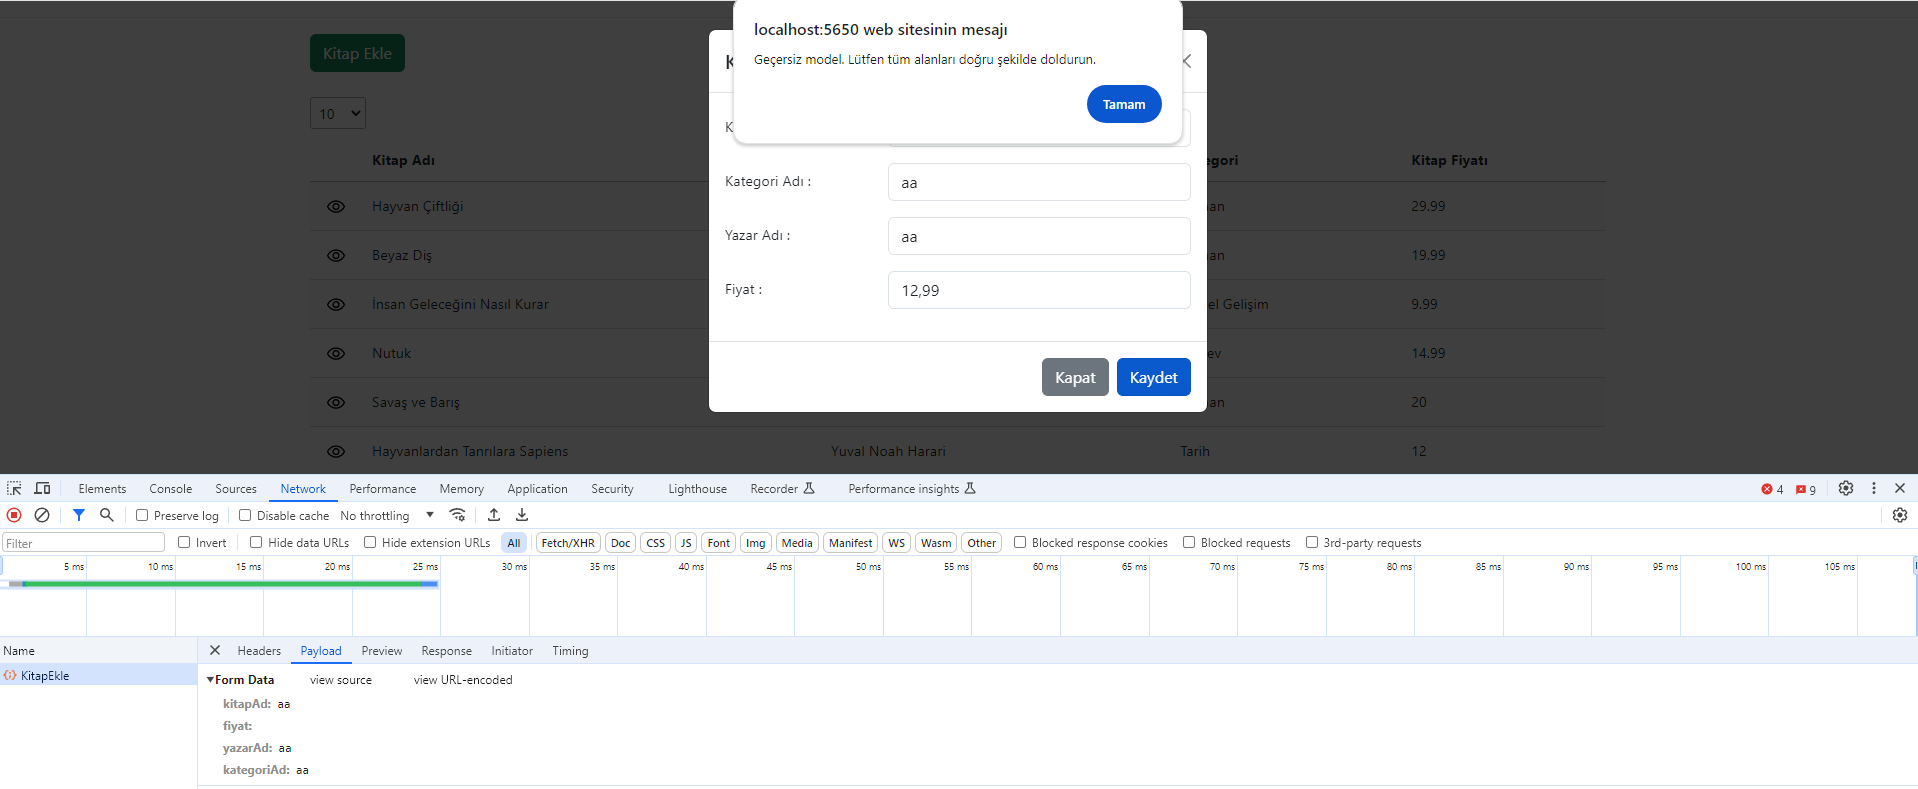
\includegraphics[ width=\textwidth, height=8cm]{kitapEkleHata.png} 
	\caption{Hata}
	\label{fig:type}
\end{figure}

 \newpage
\section{Ekleme İşleminin Gerçekleştirilmesi}
 Geçtiğimiz aylarda, Türkiye Cumhuriyeti hükümeti tarafından alınan karar doğrultusunda, uluslararası platformlarda "Turkey" yerine "Türkiye" isminin kullanılması kararlaştırılmıştır. Bu kararın ardından, teknoloji şirketleri de yazılımlarında bu değişikliği yansıtmak üzere güncellemeler yapmaya başlamıştır. Özellikle Microsoft, Windows işletim sisteminde bu değişikliği uygulamış ve "Turkey" ifadelerini "Türkiye" olarak güncellemiştir. Bu kapsamda, 22H2 sürüm numarasına sahip Windows 11 güncellemesi (22621.2715), Türkiye'nin adının doğru bir şekilde yansıtılması amacıyla yayımlanmıştır. Ancak, bu güncelleme sonrası, bazı yazılım ve kodlarda "Turkey" ifadesine bağlı olarak çalışan sistemlerde hatalar meydana gelmiştir.
 Hatayı bulmama yardımcı olan adres \cite{badem2024}. \newline
Bu isim değişikliğinin ardından, yazılım projemde çeşitli hatalar meydana gelmiştir. Sorunun kaynağını araştırdığımda, PostgreSQL veritabanımda yer alan tablolarımın bazı parametrelerinin veri tiplerini yeniden tanımlamam gerektiğini fark ettim. Bu süreçte tüm verilerimi dışa aktarıp, PostgreSQL’i tamamen silip yeniden yükledim. Verilerimi tekrar yüklerken, bazı sütunların veri tiplerini "identity always" olarak tanımlamam gerektiğini unutmuşum. Bu eksiklik, yeni veri ekleme işlemleri sırasında her yeni kaydın 1'den başlamasına ve böylece aslında mevcut olan benzersiz değerlere çakışmasına neden olmuştur. Sonuç olarak, bu durum kodumda hatalara yol açmış ve projemin düzgün çalışmasını engellemiştir. Bu deneyim, veritabanı yapılandırmalarının ve veri tiplerinin doğru tanımlanmasının yazılım projelerinin sürdürülebilirliği açısından ne denli kritik olduğunu göstermiştir. Ekleme işlemini gerçekleştirirken \cite{chatgpt} yararlanılmıştır.

\newpage
\section{Silme İşleminin Gerçekleştirilmesi}
Kitap detay butonunda aktif hale gelen pencere içerisinde silme işlemi gerçekleştirildi. Bu işlem, kullanıcıların mevcut kitapları veritabanından silmelerine olanak tanır ve kullanıcı dostu bir arayüz sağlamak amacıyla dikkatlice ele alındı. Kullanıcı, kitap listesinde yer alan bir kitabın detaylarını görmek için ilgili kitap satırındaki detay butonuna tıklayarak kitap detay penceresini aktif hale getirir. Detay penceresinde bulunan sil butonuna tıklayarak kitap silme işlemi başlatılır ve onay verilirse arka planda silme işlemi başlar. Veritabanı katmanında, PostgreSQL'de gerekli fonksiyonlar yazıldı ve bu fonksiyonlar kitap id'sine göre kitabın güvenli bir şekilde silinmesini sağlar. İşlem başarılı bir şekilde tamamlandığında, kullanıcıya işlem sonucunu bildiren geri bildirim mesajı gösterilir ve bu mesaj, belirli bir süre ekranda kalıp otomatik olarak kaybolur, böylece arayüz daha temiz ve kullanıcı dostu hale gelir. Kullanıcının karşılaşabileceği hataları daha iyi anlaması için hata mesajları da detaylandırıldı ve çeşitli senaryolar altında test edilerek kullanıcı etkileşimlerinin düzgün çalıştığından ve geri bildirim mesajlarının doğru zamanda ve doğru şekilde gösterildiğinden emin olundu. Bu iyileştirmeler, kullanıcıların kitapları yönetirken daha sorunsuz bir deneyim yaşamalarını sağlar ve uygulamanın genel kullanıcı deneyimini iyileştirir.

\begin{figure}[htbp]
	\centering
	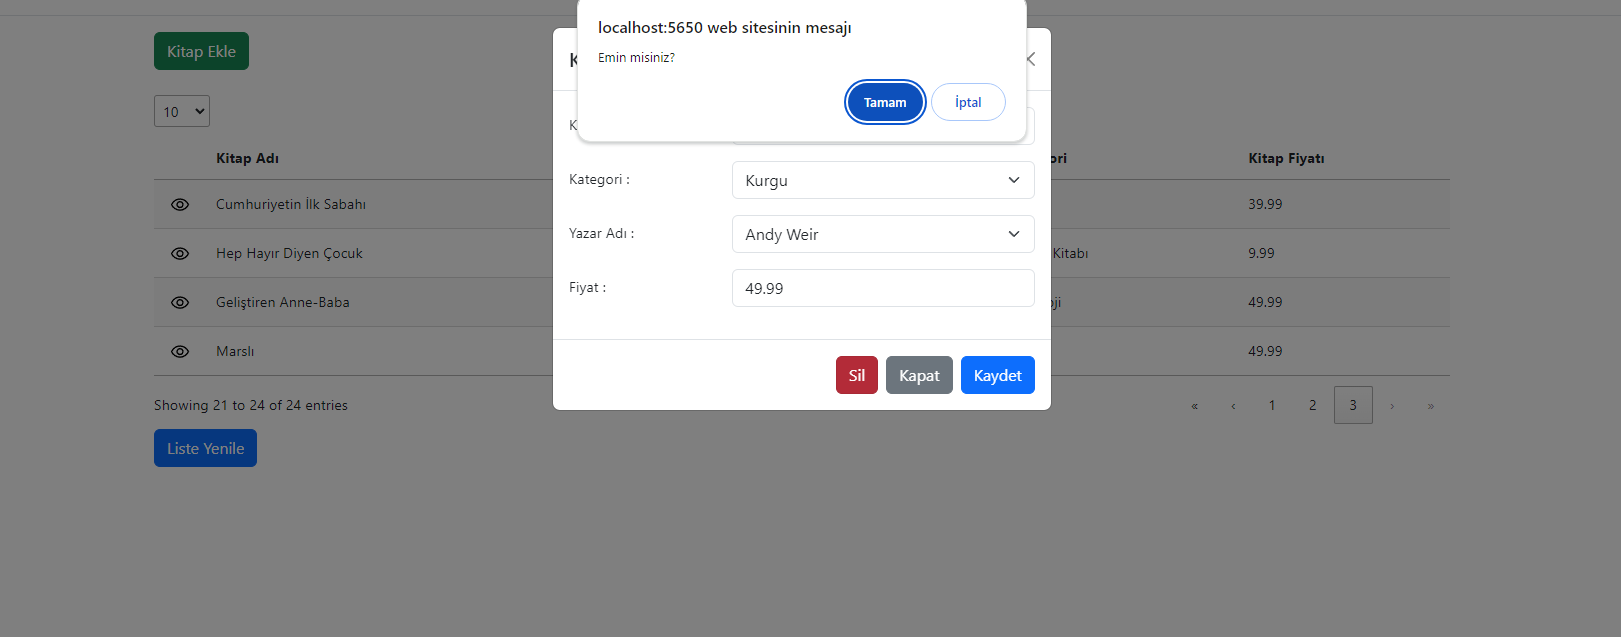
\includegraphics[ width=\textwidth, height=9cm]{sil_islem.png} 
	\caption{Silme İşlemi}
	\label{fig:type}
\end{figure}

\newpage
\begin{thebibliography}{9}
	\bibitem{kanal:isim} Murat Yücedağ, "Murat Yücedağ YouTube Kanalı", YouTube. \url{https://www.youtube.com/MurattYucedag}
	\bibitem{chatgpt} ChatGPT, OpenAI. \url{https://openai.com/gpt}
	\bibitem{bootstrap} The Bootstrap Authors. \url{https://getbootstrap.com/}
	\bibitem{datatables} DataTables. \url{https://datatables.net/}
	\bibitem{badem2024} Halil Han Badem. \textit{PostgreSQL'de Türkiye Sorunu ve Windows Güncellemesi}. 2024. \url{https://tr.linkedin.com/pulse/postgresqlde-t%C3%BCrkiye-sorunu-windows-g%C3%BCncellemesi-halil-han-badem-7kxhf}. 
	\bibitem{jivochat2024}  \textit{Pop-up Nedir?}. 2024. \url{https://www.jivochat.com.tr/blog/araclar/popup-nedir.html}.
		
\end{thebibliography}
\newpage
	
\end{document}	